\documentclass[aspectratio=169, 9pt]{beamer}

\usepackage[utf8]{inputenc}
\usepackage[T1]{fontenc}
\usepackage[brazil]{babel}
\usepackage{booktabs}
\usepackage{colortbl}
\usepackage{xcolor}
\usepackage{amsmath}
\usepackage{tikz}
\usetikzlibrary{arrows.meta, positioning, fit, calc}
\usepackage{pgfplots}
\pgfplotsset{compat=1.18}
\usepackage{fontawesome5}

\usetheme{metropolis}
\metroset{block=fill, progressbar=frametitle, numbering=fraction}

\definecolor{azul}{RGB}{25,90,160}
\definecolor{verde}{RGB}{30,140,70}
\definecolor{vermelho}{RGB}{200,40,40}
\definecolor{amarelo}{RGB}{220,160,0}
\definecolor{cinza}{RGB}{120,120,120}

\setbeamercolor{normal text}{fg=black!85}
\setbeamercolor{frametitle}{bg=azul, fg=white}
\setbeamercolor{progress bar}{fg=verde}
\setbeamercolor{alerted text}{fg=vermelho}
\setbeamercolor{example text}{fg=verde}
\setbeamercolor{block title}{bg=azul!15, fg=azul}
\setbeamercolor{block body}{bg=azul!5}
\setbeamercolor{block title alerted}{bg=vermelho!15, fg=vermelho}
\setbeamercolor{block body alerted}{bg=vermelho!5}
\setbeamercolor{block title example}{bg=verde!15, fg=verde!60!black}
\setbeamercolor{block body example}{bg=verde!5}

\title{Pseudo-Rotulagem Fraca para reconhecimento de entidades em relatos do Disque Denúncia}
\subtitle{Tema 6 --- Machine Learning}
\author{}
\date{Junho de 2026}

\begin{document}

\maketitle

\begin{frame}{O Problema: Poucos Dados, Muitos Relatos}

  \begin{columns}[T]
    \begin{column}{.50\textwidth}

      \textbf{O Disque Denúncia recebe relatos diariamente:}\\[6pt]

      \begin{tikzpicture}
        \fill[azul!10, rounded corners=4pt]   (0,0)   rectangle (6.7, 1.0);
        \fill[verde!10, rounded corners=4pt]  (0,1.2) rectangle (6.7, 2.2);

        \node[anchor=west, font=\small] at (0.2, 0.50) {%
          \textcolor{azul}{\faLock}~\textbf{DDsmall:} 5.230 relatos \emph{anotados manualmente}};
        \node[anchor=west, font=\small] at (0.2, 1.70) {%
          \textcolor{verde}{\faDatabase}~\textbf{DDlarge:} 184.493 relatos \emph{sem anotação}};
      \end{tikzpicture}

      \vspace{10pt}
      \textbf{Por que anotar manualmente é um problema?}
      \begin{itemize}
        \item Especialista lê relato por relato
        \item Marca cada Pessoa, Local e Organização
        \item Processo \alert{caro}, \alert{lento} e \alert{não escalável}
        \item 184 mil relatos não anotados ficam inutilizados
      \end{itemize}
    \end{column}

    \begin{column}{.46\textwidth}
      \begin{exampleblock}{Exemplo de relato anotado}
        \footnotesize
        ``\textit{\ldots\,%
        \textcolor{azul!80!black}{\underline{Ruan}}
        foi visto armado na
        \textcolor{verde!70!black}{\underline{Tijuca}}
        com integrantes da
        \textcolor{amarelo!80!black}{\underline{polícia}}.
        Segundo moradores de
        \textcolor{verde!70!black}{\underline{São Gonçalo}}\ldots}''
      \end{exampleblock}

      \vspace{6pt}
      {\footnotesize
      \textcolor{azul!80!black}{\rule{8pt}{6pt}}~Pessoa \quad
      \textcolor{verde!70!black}{\rule{8pt}{6pt}}~Local \quad
      \textcolor{amarelo!80!black}{\rule{8pt}{6pt}}~Organização
      }

      \vspace{10pt}
      \begin{alertblock}{Dificuldades do domínio}
        \begin{itemize}
          \item Linguagem informal e abreviações (\emph{pm, cv, tcp})
          \item Variações ortográficas (\emph{polícia / policia})
          \item Apelidos (\emph{``Ruan''}, \emph{``Mara''})
          \item Entidades ambíguas (\emph{``Batalhão''})
        \end{itemize}
      \end{alertblock}
    \end{column}
  \end{columns}
\end{frame}


\begin{frame}{Pergunta de Pesquisa e Hipótese}
  \begin{block}{Hipótese do trabalho}
    Se uma entidade apareceu anotada no conjunto pequeno, ela pode reaparecer na base grande e gerar exemplos adicionais de treino. Isso pode expor o modelo a \textbf{mais contextos reais} e melhorar sua \textbf{generalização}.
  \end{block}

  \vspace{10pt}
  \begin{center}
  \begin{tikzpicture}[
    caixa/.style={rounded corners=4pt, draw=azul!70, fill=azul!10, minimum height=11mm, text width=34mm, align=center, font=\small, very thick},
    caixaV/.style={rounded corners=4pt, draw=verde!70!black, fill=verde!10, minimum height=11mm, text width=34mm, align=center, font=\small, very thick},
    seta/.style={-{Stealth[length=5pt]}, very thick, azul!70}
  ]
    \node[caixa] (a) at (0,0) {Lista de entidades\\já conhecidas};
    \node[caixaV] (b) at (4.7,0) {Busca automática\\na base grande};
    \node[caixa] (c) at (9.4,0) {Novos exemplos\\para treino};
    \draw[seta] (a) -- (b);
    \draw[seta] (b) -- (c);
  \end{tikzpicture}
  \end{center}

  \vspace{10pt}
  \begin{exampleblock}{Formulação da proposta}
    Em vez de marcar tudo do zero, o trabalho tenta \textbf{reaproveitar o que já foi aprendido no DDsmall} para gerar novas marcações no DDlarge.
  \end{exampleblock}
\end{frame}

\begin{frame}{Etapa 1 -- Extração do Léxico}
  \begin{columns}[T]
    \begin{column}{.53\textwidth}
      \textbf{De onde veio essa lista?}\\[4pt]
      Apenas do \textbf{treino do DDsmall}, com \textbf{4.226 relatos}.

      \vspace{8pt}
      \begin{itemize}
        \item O texto já anotado foi percorrido relato por relato.
        \item Cada entidade marcada entrou em uma lista.
        \item Essa lista virou o ponto de partida do experimento.
      \end{itemize}
    \end{column}

    \begin{column}{.43\textwidth}
      \begin{exampleblock}{Exemplo de lista}
        \footnotesize
        Ruan $\rightarrow$ Pessoa\\
        Tijuca $\rightarrow$ Local\\
        São Gonçalo $\rightarrow$ Local\\
        polícia $\rightarrow$ Organização
      \end{exampleblock}

      \vspace{6pt}
      \small
      A ideia aqui não era inventar entidades novas, e sim reunir as que já apareciam anotadas no conjunto de treino.
    \end{column}
  \end{columns}
\end{frame}


\begin{frame}{Etapa 2 -- Filtragem do Léxico}

\begin{columns}[T]

%%%%%%%%%%%%%%%%%%%%%%%%%%%%%%%%%%%%%%%%%%
\begin{column}{0.33\textwidth}

\begin{block}{Por que filtrar?}
Grande parte das entidades aparecia muito poucas vezes no conjunto de treino, aumentando o risco de pseudo-anotações incorretas.
\end{block}

\vspace{5pt}

\begin{itemize}
\item Léxico inicial: \textbf{5.899 entidades}
\item Removidas entidades com frequência $\leq 2$
\item Mantidas apenas entidades mais recorrentes
\end{itemize}

\vspace{8pt}

\begin{exampleblock}{Resultado}
\centering

\Large
\textbf{5.899}

\vspace{2pt}

$\Longrightarrow$

\vspace{2pt}

{\color{verde!70!black}\Huge\textbf{1.057}}

\vspace{3pt}

\normalsize
entidades no léxico final

\end{exampleblock}

\end{column}

%%%%%%%%%%%%%%%%%%%%%%%%%%%%%%%%%%%%%%%%%%
\begin{column}{0.64\textwidth}

\centering
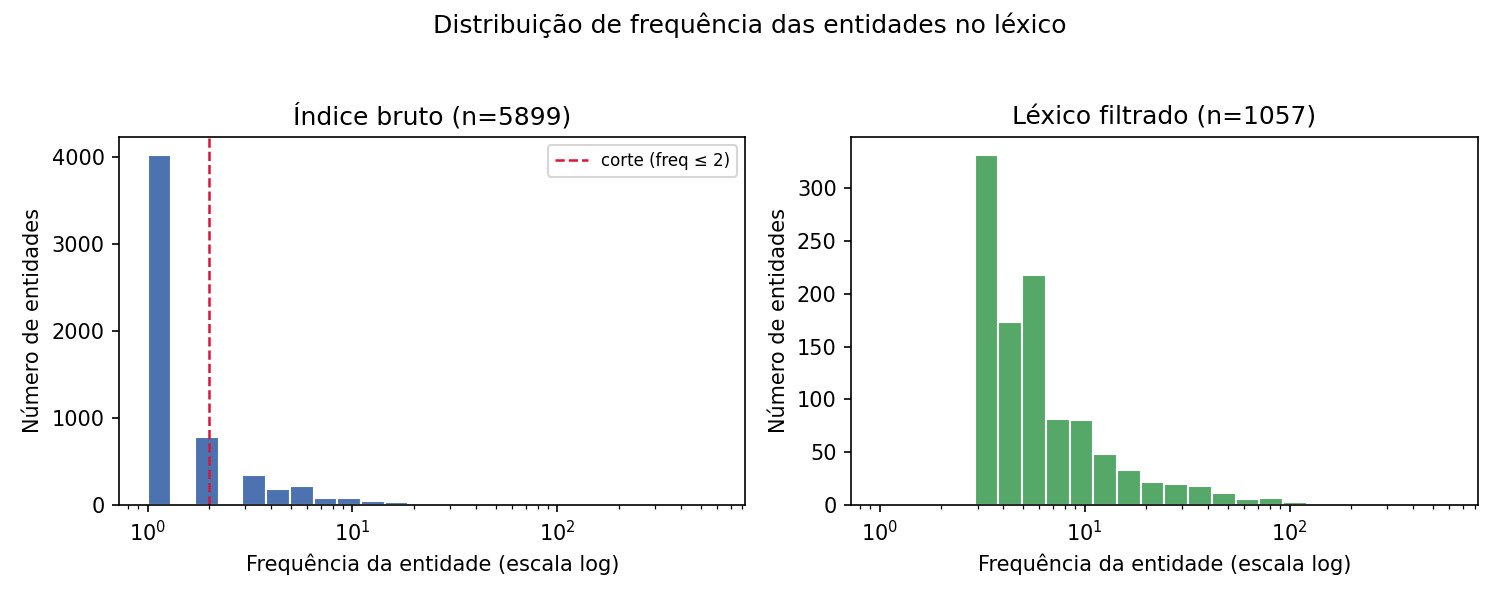
\includegraphics[width=\linewidth]{etapa2.jpeg}

\vspace{2mm}

{\scriptsize
A linha vermelha representa o corte adotado (frequência > 2). Observa-se que a maioria das entidades ocorria apenas uma ou duas vezes, sendo removida para reduzir o ruído do léxico.
}

\end{column}

\end{columns}

\end{frame}

\begin{frame}{Etapa 3 -- Projeção Lexical sobre o DDlarge}
  \begin{block}{O que é a projeção lexical?}
    É usar a lista de entidades conhecidas para procurar essas mesmas entidades nos relatos ainda não anotados.
  \end{block}

  \vspace{8pt}
  \begin{columns}[T]
    \begin{column}{.47\textwidth}
      \begin{exampleblock}{Exemplo de lista}
        \footnotesize
        Ruan $\rightarrow$ Pessoa\\
        Tijuca $\rightarrow$ Local\\
        polícia $\rightarrow$ Organização
      \end{exampleblock}
    \end{column}

    \begin{column}{.47\textwidth}
      \begin{exampleblock}{Relato do DDlarge}
        \footnotesize
        ``Ruan foi visto na Tijuca com integrantes da polícia.''
      \end{exampleblock}
    \end{column}
  \end{columns}

  \vspace{8pt}
  \begin{alertblock}{Procedimento}
    Ele encontra automaticamente as ocorrências conhecidas e cria as marcações sem intervenção humana.
  \end{alertblock}
\end{frame}

\begin{frame}{Etapa 4 -- Construção do Corpus Pseudo-anotado}
  \begin{columns}[T]
    \begin{column}{.48\textwidth}
      \textbf{Depois da busca automática, alguns relatos do DDlarge passaram a ter marcações.}\\[8pt]

      Esses relatos formaram um novo conjunto de treino auxiliar: o \textbf{corpus pseudo-anotado}.

      \vspace{8pt}
      \begin{exampleblock}{Natureza dos pseudo-rótulos}
        As marcações não foram feitas por pessoas.\\[4pt]
        Elas foram geradas pelo algoritmo a partir da lista de entidades.
      \end{exampleblock}
    \end{column}

    \begin{column}{.46\textwidth}
      \begin{block}{Resultado da projeção}
        \centering
        \Large \textbf{133.841 relatos}\\[4pt]
        \normalsize com pelo menos uma marcação automática

        \vspace{8pt}
        \Large \textbf{450.833 entidades}\\[4pt]
        \normalsize no total
      \end{block}

      \vspace{8pt}
      \small
      A projeção atingiu \textbf{72,5\%} do DDlarge. O léxico ficou mais restrito depois da Etapa 2, então a cobertura caiu, mas a qualidade de cada marcação melhorou.
    \end{column}
  \end{columns}
\end{frame}

\begin{frame}{Modelos e Configurações Comparadas}
  \begin{center}
  \begin{tikzpicture}[
    caixaA/.style={rounded corners=4pt, draw=azul!70, fill=azul!10, text width=38mm, align=center, minimum height=10mm, font=\small, very thick},
    caixaB/.style={rounded corners=4pt, draw=verde!70!black, fill=verde!10, text width=38mm, align=center, minimum height=10mm, font=\small, very thick},
    setaA/.style={-{Stealth[length=5pt]}, thick, azul!70},
    setaB/.style={-{Stealth[length=5pt]}, thick, verde!70!black}
  ]
    \node[font=\small\bfseries, text=azul] at (-4.2,2.5) {Baseline};
    \node[caixaA] (b1) at (-4.2,1.4) {DDsmall};
    \node[caixaA] (b2) at (-4.2,0.0) {Modelo treinado};
    \draw[setaA] (b1) -- (b2);

    \node[font=\small\bfseries, text=verde!60!black] at (4.2,2.5) {Proposta};
    \node[caixaB] (p1) at (4.2,1.8) {DDsmall};
    \node[caixaB] (p2) at (4.2,0.6) {+ pseudo-anotado};
    \node[caixaB] (p3) at (4.2,-0.8) {Modelo treinado};
    \draw[setaB] (p1) -- (p2);
    \draw[setaB] (p2) -- (p3);

    \node[draw=vermelho, very thick, rounded corners=4pt, fill=vermelho!8, text width=42mm, align=center, minimum height=10mm, font=\small] (teste) at (0,-2.6) {Mesma avaliação final\\no conjunto de teste};
    \draw[-{Stealth[length=5pt]}, thick, vermelho!70] (b2.south) |- (teste.west);
    \draw[-{Stealth[length=5pt]}, thick, vermelho!70] (p3.south) |- (teste.east);
  \end{tikzpicture}
  \end{center}

  \vspace{4pt}
  \small
  Configurações mínimas avaliadas: \textbf{Baseline 1} pré-treinado, \textbf{Baseline 2} treinado só no DDsmall, \textbf{Proposta 1} com EntityRuler e \textbf{Proposta 2} com DDsmall + pseudo-anotado.\\[4pt]
  Entre as variantes da Proposta 2, a configuração com \textbf{20k exemplos pseudo-anotados} foi a melhor; por isso ela entrou na comparação principal.\\[4pt]
  A comparação central foi: \textbf{treinar com o pseudo-anotado melhora o desempenho em relação ao treino apenas com o conjunto anotado manualmente?}
\end{frame}

\begin{frame}{Avaliação em nível de entidade, todas as configurações}
  \small
  Uma predição só é considerada correta quando o \textbf{span} e a \textbf{classe} coincidem exatamente com o gabarito.

  \vspace{6pt}
  \centering
  \scriptsize
  \begin{tabular}{lccc|ccc|ccc|c}
    \toprule
    & \multicolumn{3}{c}{\textbf{Pessoa}} & \multicolumn{3}{c}{\textbf{Localização}} & \multicolumn{3}{c}{\textbf{Organização}} & \\
    \textbf{Modelo} & P & R & F1 & P & R & F1 & P & R & F1 & \textbf{micro-F1} \\
    \midrule
    Baseline 2 (DDsmall)     & 0,749 & 0,722 & 0,735 & 0,834 & 0,828 & 0,831 & 0,749 & 0,750 & 0,749 & \textbf{0,795} \\
    Proposta 2 (20k)         & 0,589 & 0,441 & 0,504 & 0,815 & 0,658 & 0,729 & 0,692 & 0,691 & 0,692 & 0,676 \\
    Proposta 1 (EntityRuler) & 0,552 & 0,406 & 0,468 & 0,830 & 0,591 & 0,690 & 0,687 & 0,671 & 0,679 & 0,642 \\
    Proposta 2 (completo)    & 0,535 & 0,398 & 0,457 & 0,828 & 0,596 & 0,693 & 0,723 & 0,640 & 0,679 & 0,641 \\
    Baseline 1 (zero-shot)   & 0,408 & 0,495 & 0,447 & 0,409 & 0,347 & 0,375 & 0,254 & 0,149 & 0,187 & 0,362 \\
    \bottomrule
  \end{tabular}

  \vspace{8pt}
  \small
  O \textbf{Baseline 2} tem o melhor micro-F1. A \textbf{Proposta 1}, baseada só em regras, fica praticamente empatada com a \textbf{Proposta 2 completa}, 0,642 contra 0,641: usar mais dados pseudo-anotados não trouxe ganho adicional sobre o teto de um sistema de regras puro.
\end{frame}

\begin{frame}{Avaliação principal}
  \begin{block}{Como a avaliação foi feita}
    Todas as métricas abaixo foram medidas no \textbf{teste do DDsmall}, em \textbf{nível de entidade}: uma predição só conta como correta quando \textbf{span e classe} coincidem com o o rótulo verdadeiro.
  \end{block}

  \vspace{4pt}
  \centering
  \scriptsize
  \begin{tabular}{lccc|ccc}
    \toprule
    & \multicolumn{3}{c|}{\textbf{Baseline 2}} & \multicolumn{3}{c}{\textbf{Proposta 2 (20k)}} \\
    \textbf{Classe} & \textbf{P} & \textbf{R} & \textbf{F1} & \textbf{P} & \textbf{R} & \textbf{F1} \\
    \midrule
    Pessoa & 0,749 & 0,722 & 0,735 & 0,589 & 0,441 & 0,504 \\
    Local & 0,834 & 0,828 & 0,831 & 0,815 & 0,658 & 0,729 \\
    Organização & 0,749 & 0,750 & 0,749 & 0,692 & 0,691 & 0,692 \\
    \midrule
    Micro & 0,800 & 0,791 & 0,795 & 0,745 & 0,620 & 0,676 \\
    Macro F1 & -- & -- & 0,772 & -- & -- & 0,641 \\
    \bottomrule
  \end{tabular}

  \vspace{6pt}
  \begin{columns}[T]
    \begin{column}{.48\textwidth}
      \begin{exampleblock}{Contagem de erros}
        \small
        Baseline 2: \textbf{605 FP}, \textbf{639 FN}, \textbf{119 erros de classe}.\\[2pt]
        Proposta 2 (20k): \textbf{650 FP}, \textbf{1.163 FN}, \textbf{83 erros de classe}.
      \end{exampleblock}
    \end{column}
    \begin{column}{.48\textwidth}
      \begin{block}{Maior impacto por classe}
        \small
        \textbf{Pessoa} teve a maior queda de F1, de \textbf{0,735} para \textbf{0,504}. \textbf{Organização} foi a classe que caiu menos, de \textbf{0,749} para \textbf{0,692}.
      \end{block}
    \end{column}
  \end{columns}
\end{frame}

\begin{frame}{Léxico e pseudo-anotação}
  \begin{columns}[T]
    \begin{column}{.49\textwidth}
      \begin{block}{Léxico extraído do treino}
        \small
        \textbf{5.899} entidades brutas; \textbf{1.057} mantidas; \textbf{4.842} removidas.

        \vspace{4pt}
        Por classe: Local \textbf{662}, Pessoa \textbf{248}, Organização \textbf{147}.

        \vspace{4pt}
        Mantidos: \textit{polícia}, \textit{São Gonçalo}, \textit{rj}, sigla de exceção.\\
        Removidos: \textit{sg}, \textit{Fernando beira mar}, \textit{Flamengo}, \textit{Botafogo}.
      \end{block}
    \end{column}

    \begin{column}{.49\textwidth}
      \begin{exampleblock}{Pseudo-anotação no DDlarge}
        \small
        \textbf{133.841 relatos} pseudo-anotados\\
        \textbf{450.833 pseudo-entidades}

        \vspace{4pt}
        Por classe: Local \textbf{236.763}, Organização \textbf{142.636}, Pessoa \textbf{71.434}.
      \end{exampleblock}

      \begin{alertblock}{Inspeção manual da amostra}
        \small
        Houve casos plausíveis, como \textit{São Gonçalo} e \textit{Jardim Catarina} marcados como \textbf{Local}.\\[2pt]
        Mas também surgiram termos ambíguos, como \textit{posse} e \textit{PROVIDENCIA} marcados como Local fora de contexto.
      \end{alertblock}

      \vspace{3pt}
      \small
      A projeção lexical \textbf{não usa contexto}: o mesmo termo tende a receber o mesmo rótulo mesmo em usos ambíguos.
    \end{column}
  \end{columns}
\end{frame}

\begin{frame}{Resultado principal}
  \begin{columns}[T]
    \begin{column}{.58\textwidth}
      \begin{center}
      \begin{tikzpicture}
      \begin{axis}[
        ybar=6pt,
        width=7.6cm,
        height=6.0cm,
        ymin=0,
        ymax=1.0,
        ylabel={F1 micro},
        symbolic x coords={{Baseline 2},{Proposta 2 20k}},
        xtick=data,
        nodes near coords,
        nodes near coords style={font=\small\bfseries},
        bar width=24pt,
        enlarge x limits=0.35,
        grid=major,
        grid style={dashed, gray!30},
        tick label style={font=\small},
      ]
      \addplot[fill=verde!70, draw=verde!80!black] coordinates {({Baseline 2},0.795)};
      \addplot[fill=vermelho!60, draw=vermelho!80!black] coordinates {({Proposta 2 20k},0.676)};
      \end{axis}
      \end{tikzpicture}
      \end{center}
    \end{column}

    \begin{column}{.38\textwidth}
      \begin{alertblock}{Síntese dos resultados}
        A hipótese \textbf{não foi confirmada}.\\[4pt]
        O modelo com pseudo-rótulos ficou abaixo do baseline supervisionado.
      \end{alertblock}

      \vspace{8pt}
      \small
      Entre as configurações mínimas, o melhor resultado ficou com o \textbf{Baseline 2}. A pseudo-anotação não melhorou a generalização no teste, e a queda foi especialmente forte em \textbf{Pessoa}, enquanto \textbf{Organização} caiu menos.
    \end{column}
  \end{columns}
\end{frame}

\begin{frame}{Interpretação dos Erros}
  \begin{columns}[T]
    \begin{column}{.48\textwidth}
      \begin{block}{1. Entidades fora do léxico dispararam}
        Os \textbf{falsos negativos fora do léxico} passaram de \textbf{188} no Baseline 2 para \textbf{557} na Proposta 2 (20k).\\[2pt]
        O léxico ficou bem menor depois da Etapa 2, então muitas entidades legítimas nunca chegaram a ser pseudo-anotadas.
      \end{block}

      \vspace{6pt}
      \begin{block}{2. Variantes ortográficas continuaram difíceis}
        Os \textbf{falsos negativos por variação ortográfica} subiram de \textbf{68} para \textbf{219}.\\[2pt]
        O pseudo-corpus reforça as formas exatas do léxico, e o léxico agora cobre menos variantes de cada entidade.
      \end{block}
    \end{column}

    \begin{column}{.48\textwidth}
      \begin{alertblock}{3. Entidades compostas fragmentaram mais}
        O erro \textbf{composta\_parcial} quase dobrou: de \textbf{110} para \textbf{217}.\\[2pt]
        Exemplo: \textit{morro do canta galo} reconhecido só como \textit{canta galo}.
      \end{alertblock}

      \vspace{8pt}
      \small
      Os \textbf{falsos positivos} quase não mudaram (\textbf{264} $\rightarrow$ \textbf{296}): o filtro de frequência mínima da Etapa 2 já limita a entrada de termos ambíguos no léxico. O \textbf{erro de classe} até melhorou (\textbf{119} $\rightarrow$ \textbf{83}). O problema da Proposta 2 não é ruído: é \textbf{perda de cobertura}.
    \end{column}
  \end{columns}
\end{frame}

\begin{frame}{Conclusões}
  \begin{block}{Síntese do estudo}
    O trabalho investigou se a projeção lexical sobre o DDlarge poderia gerar exemplos adicionais de treino e melhorar a generalização do modelo.
  \end{block}

  \vspace{8pt}
  \begin{block}{Síntese dos achados}
    A resposta foi \textbf{negativa}: o filtro de frequência mínima do léxico reduziu bastante o ruído, mas isso custou \textbf{cobertura}, e essa perda de cobertura piorou o modelo em vez de melhorá-lo.
  \end{block}

  \vspace{8pt}
  \begin{exampleblock}{Conclusão geral}
    A hipótese não foi confirmada. O principal resultado não é apenas esse, mas entender \textbf{por que} ela falhou: a projeção lexical decide marcar uma entidade só por correspondência exata de texto, sem usar contexto. Um léxico mais restrito reduz o ruído, mas também reduz a cobertura, e foi essa perda de cobertura que impediu a Proposta 2 de superar o baseline supervisionado.
  \end{exampleblock}
\end{frame}

\begin{frame}[standout]
  Obrigado!\\[8pt]
  \large Dúvidas?
\end{frame}

\end{document}